\documentclass[11pt,a4paper]{article}
\usepackage[utf8]{inputenc}
\usepackage[T1]{fontenc}
\usepackage{geometry}
\geometry{a4paper, margin=1in}
\usepackage{setspace}
\onehalfspacing
\usepackage{float}
\usepackage{xcolor}
\usepackage{hyperref}
\hypersetup{colorlinks=true, linkcolor=blue!50!black, urlcolor=blue!50!black}
\usepackage{booktabs}
\usepackage{array}
\usepackage{tabularx}
\usepackage{fancyhdr}
\usepackage{tikz}
\usetikzlibrary{shapes.geometric, shapes.multipart, arrows.meta, positioning, fit, calc, backgrounds}

\setlength{\headheight}{14pt}
\pagestyle{fancy}
\fancyhf{}
\fancyhead[L]{\small Task 2: Process Model \& Design -- RijalMap}
\fancyhead[R]{\small \thepage}
\renewcommand{\headrulewidth}{0.4pt}

% palette (muted, light-mode, as planned for the UI)
\definecolor{sage}{HTML}{5E8F63}
\definecolor{amberc}{HTML}{D39A2C}
\definecolor{terra}{HTML}{BC4F44}
\definecolor{greyc}{HTML}{8E8E8E}
\definecolor{paper}{HTML}{FBFBFA}
\definecolor{ink}{HTML}{2B2B2B}

\tikzset{
  box/.style={draw=ink, rounded corners=2pt, fill=paper, align=center, font=\footnotesize\sffamily, inner sep=5pt},
  arr/.style={-{Stealth[length=2.2mm]}, thick, draw=ink},
  entity/.style={draw=ink, rectangle split, rectangle split parts=2, rectangle split part fill={black!10,paper},
     align=left, font=\scriptsize\sffamily, inner sep=4pt, text width=3.4cm},
  cls/.style={draw=ink, rectangle split, rectangle split parts=3, rectangle split part fill={black!10,paper,paper},
     align=left, font=\scriptsize\sffamily, inner sep=3pt, text width=4.0cm},
  lab/.style={font=\scriptsize\sffamily, fill=white, inner sep=1pt},
}

\newcommand{\actor}[3]{%
  \draw[ink, thick] (#1,#2+0.95) circle (0.15);
  \draw[ink, thick] (#1,#2+0.8)--(#1,#2+0.35);
  \draw[ink, thick] (#1-0.25,#2+0.65)--(#1+0.25,#2+0.65);
  \draw[ink, thick] (#1,#2+0.35)--(#1-0.2,#2);
  \draw[ink, thick] (#1,#2+0.35)--(#1+0.2,#2);
  \node[font=\scriptsize\sffamily, align=center] at (#1,#2-0.45) {#3};}

\begin{document}

\begin{center}
    {\Large \textbf{Task 2 -- Mini Project 1: Software Process Model and Design}}\\[0.25cm]
    {\large CS4525 Software Engineering}\\[0.25cm]
    {\large \textbf{RijalMap: The Intelligent Isnad Visualizer}}\\[0.25cm]
    Submitted by: Muhammad Jahanzaib Bhutta (Roll No. 0001127586)\\
    BS Artificial Intelligence, Allama Iqbal Open University\\
    Supervisor: Ma'am Kashia Riaz\\
    \textbf{Individual submission} (one student, no group) \quad|\quad November 2026
\end{center}
\vspace{0.2cm}

%--------------------------------------------------------------
\section{Project Summary and Requirements}
%--------------------------------------------------------------
\subsection{Problem and goal}
A hadith reaches us through a chain of narrators (\emph{isnad}). Checking a chain by hand means looking up every narrator and every teacher--student pair in rijal books, and the same narrators appear in thousands of chains across many books. RijalMap lets a user pick a book and a hadith number, and then draws the narrators of that hadith as a directed graph. Each link between two narrators is coloured by how well the available data supports it. The tool is a visual aid for checking chains. It does not grade narrators or hadith, and it makes no \emph{sahih/da'if} ruling.

\subsection{Data sources and what I measured}
I use two public Kaggle datasets by the same author, which are linked by one key: \texttt{chain\_indx} in the hadith dataset refers to \texttt{scholar\_indx} in the narrators dataset~\cite{narrators,hadiths}. Before designing the database I profiled both files in pandas. The results shaped the design (Table~\ref{tab:data}).

\begin{table}[H]
\centering
\small
\begin{tabularx}{\textwidth}{@{}Xr@{}}
\toprule
\textbf{Measurement} & \textbf{Value}\\
\midrule
Narrators dataset (\texttt{all\_rawis}): columns & 25 (about 24,000 narrators)\\
Hadith dataset: rows (one row per chain), six collections & 34,441\\
Chains with no narrator list & 0.36\%\\
Numeric birth year (\texttt{birth\_date\_hijri}) missing & 98.4\%\\
Numeric death year (\texttt{death\_date\_hijri}) missing & 83.8\%\\
Consecutive narrator pairs found in all chains & 141,377\\
\quad of which listed in a teacher or student column & 105,817 (74.8\%)\\
\bottomrule
\end{tabularx}
\caption{Facts measured from the datasets. Stated chain order: the first ID is the narrator nearest the collector and the last is the Companion (checked on Sahih al-Bukhari no.~1, whose list ends with `Umar ibn al-Khattab).}
\label{tab:data}
\end{table}

The six collections contribute 7,596 rows (Sahih Muslim), 7,370 (Sahih al-Bukhari), 5,774 (Sunan an-Nasa'i), 5,260 (Sunan Abi Da'ud), 4,227 (Sunan Ibn Majah) and 4,214 (Jami' al-Tirmidhi).

Two findings changed my original plan. First, almost no narrators have both a numeric birth and death year, so a purely date-based check would leave nearly every link undecided. Second, the teacher and student columns do record most links (74.8\%), so those columns are the main evidence, and the dates serve as a second check that can only catch clear contradictions. The numeric hijri columns also lose the sign of pre-Hijra years (the Prophet, peace be upon him, is stored with birth year 53, while the text column \texttt{birth\_date} says ``53 BH''), so the import must read years from the text columns and store BH years as negative numbers.

\subsection{Functional requirements}
\begin{enumerate}
    \item \textbf{FR1:} The user selects a collection and a hadith number.
    \item \textbf{FR2:} The system draws all chains found for that number as one directed graph (teacher $\rightarrow$ student), so shared narrators appear once.
    \item \textbf{FR3:} Every link is coloured by the rule in Table~\ref{tab:colours}, with a legend on screen.
    \item \textbf{FR4:} Clicking a link or a narrator shows the evidence: the narrators' dates, and whether the link is listed in the dictionary.
    \item \textbf{FR5 (if time allows):} The user can browse a narrator's recorded teachers and students.
\end{enumerate}
\textbf{Out of scope:} grading narrators or hadith, importing raw Arabic text and splitting names automatically, user accounts, and online deployment.

\begin{table}[H]
\centering
\small
\begin{tabularx}{\textwidth}{@{}p{2.5cm}p{2.9cm}X@{}}
\toprule
\textbf{Colour / style} & \textbf{State} & \textbf{Meaning}\\
\midrule
\textcolor{sage}{\textbf{Green, solid}} & Recorded & The dictionary lists this teacher--student pair (in either narrator's entry), and no date contradicts it.\\
\textcolor{terra}{\textbf{Red, dashed}} & Contradicted & Both dates are known and the teacher died before the student was born.\\
\textcolor{amberc}{\textbf{Amber, dashed}} & Not recorded & The dictionary does not list the pair and no date contradicts it. The link needs checking; it is not called false.\\
\textcolor{greyc}{\textbf{Grey, dotted}} & Unidentified & A narrator in the pair could not be matched to the dictionary, so nothing can be checked.\\
\bottomrule
\end{tabularx}
\caption{How a link is coloured. Red is kept for positive evidence against a link, because an incomplete dictionary is not evidence that a link is false.}
\label{tab:colours}
\end{table}

%--------------------------------------------------------------
\section{Selection of the Software Process Model}
%--------------------------------------------------------------
\textbf{Selected model:} Iterative Prototyping.

\subsection{Why I selected it}
I chose Iterative Prototyping because at the start I did not know whether the data would support my idea. My first prototype used a small hand-made dataset and tried to do too much, including recording rulings on narrators. When I explored the real datasets, I found that 98.4\% of numeric birth years were missing, so the date check I had planned could not carry the project. I narrowed the scope, replaced the grading idea with colour states based on the dictionary, and added the amber state. A linear model such as Waterfall would have locked in my first design before I saw this. I work alone, so I do not use Scrum roles or sprints.

\subsection{Phases and how they apply to RijalMap}
Each iteration builds something that runs, tests it against known chains, and uses what I learn to adjust the next one (Figure~\ref{fig:cycle}).

\begin{figure}[H]
\centering
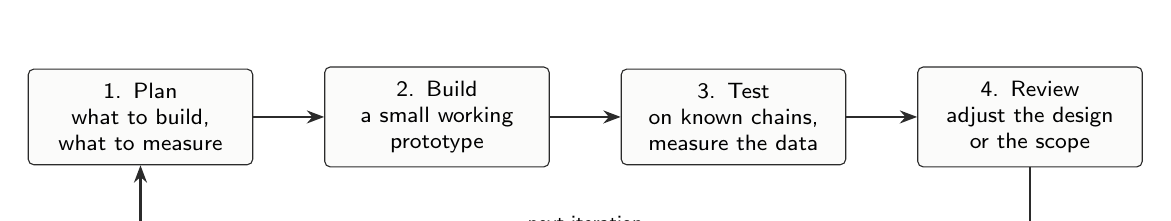
\begin{tikzpicture}[node distance=0.9cm]
  \node[box, text width=2.5cm] (a) {1. Plan\\ what to build,\\ what to measure};
  \node[box, text width=2.5cm, right=of a] (b) {2. Build\\ a small working\\ prototype};
  \node[box, text width=2.5cm, right=of b] (c) {3. Test\\ on known chains,\\ measure the data};
  \node[box, text width=2.5cm, right=of c] (d) {4. Review\\ adjust the design\\ or the scope};
  \draw[arr] (a)--(b); \draw[arr] (b)--(c); \draw[arr] (c)--(d);
  \draw[arr] (d.south) -- ++(0,-0.7) -| node[lab, pos=0.25] {next iteration} (a.south);
\end{tikzpicture}
\caption{The prototyping cycle repeated in every iteration of RijalMap.}
\label{fig:cycle}
\end{figure}

\begin{table}[H]
\centering
\small
\begin{tabularx}{\textwidth}{@{}p{0.5cm}p{3.6cm}X@{}}
\toprule
\textbf{\#} & \textbf{Iteration} & \textbf{What is built and how I check it} \\
\midrule
0 & Early prototype (done) & Hand-made seed data, PostgreSQL, console engine. It showed the scope was too wide and the data model did not match the real datasets, so I restarted. \\
1 & Data and schema & Profile both datasets, design the four tables, write the import script. \emph{Check:} row counts match the source files (34,441 hadith rows), and unmatched narrator IDs are counted and reported. \\
2 & Graph engine (console) & Build the merged graph for one hadith, classify links, find shared narrators. \emph{Check:} the output for Sahih al-Bukhari no.~1 matches the chain I verified by hand. \\
3 & API & Serve the graph as JSON through FastAPI. \emph{Check:} each endpoint in the browser test page. \\
4 & Frontend & Cytoscape.js canvas, legend, evidence panel. \emph{Check:} a single-chain and a multi-chain hadith both render correctly. \\
5 & Evaluation and report & Count how many links fall in each colour across the corpus, and write down the limits. \\
\bottomrule
\end{tabularx}
\caption{Iterations planned for RijalMap.}
\end{table}

%--------------------------------------------------------------
\section{Software Design}
%--------------------------------------------------------------
\subsection{Major components and how they interact}
The system has three layers, plus a one-time import step that fills the database (Figure~\ref{fig:arch}).

\begin{figure}[!t]
\centering
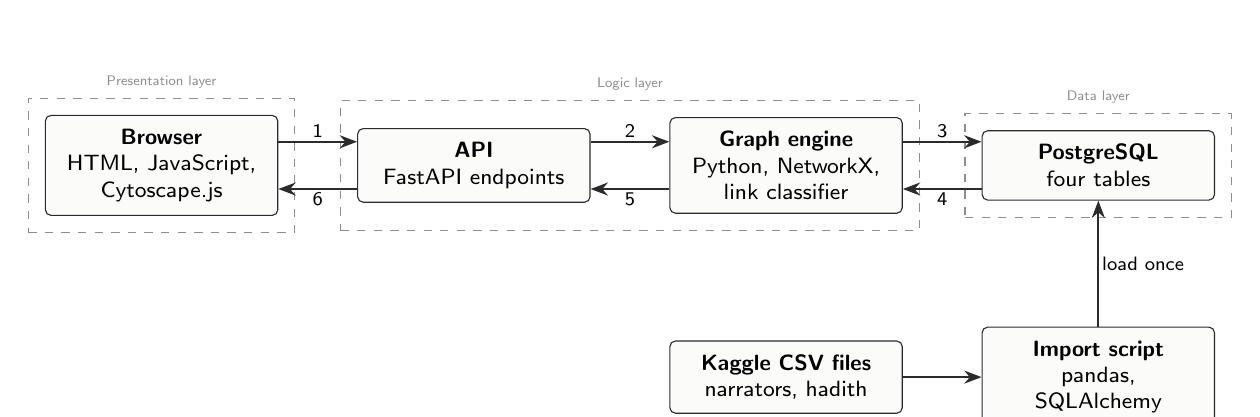
\begin{tikzpicture}
  \node[box, text width=2.6cm] (ui) {\textbf{Browser}\\ HTML, JavaScript, Cytoscape.js};
  \node[box, text width=2.6cm, right=1.0cm of ui] (api) {\textbf{API}\\ FastAPI endpoints};
  \node[box, text width=2.6cm, right=1.0cm of api] (eng) {\textbf{Graph engine}\\ Python, NetworkX, link classifier};
  \node[box, text width=2.6cm, right=1.0cm of eng] (db) {\textbf{PostgreSQL}\\ four tables};
  \node[box, text width=2.6cm, below=1.6cm of db] (imp) {\textbf{Import script}\\ pandas, SQLAlchemy};
  \node[box, text width=2.6cm, left=1.0cm of imp] (csv) {\textbf{Kaggle CSV files}\\ narrators, hadith};
  \draw[arr] ([yshift=3mm]ui.east) -- node[lab, above] {1} ([yshift=3mm]api.west);
  \draw[arr] ([yshift=-3mm]api.west) -- node[lab, below] {6} ([yshift=-3mm]ui.east);
  \draw[arr] ([yshift=3mm]api.east) -- node[lab, above] {2} ([yshift=3mm]eng.west);
  \draw[arr] ([yshift=-3mm]eng.west) -- node[lab, below] {5} ([yshift=-3mm]api.east);
  \draw[arr] ([yshift=3mm]eng.east) -- node[lab, above] {3} ([yshift=3mm]db.west);
  \draw[arr] ([yshift=-3mm]db.west) -- node[lab, below] {4} ([yshift=-3mm]eng.east);
  \draw[arr] (csv) -- (imp);
  \draw[arr] (imp) -- node[lab, right] {load once} (db);
  \begin{scope}[on background layer]
    \node[draw=greyc, dashed, fit=(ui), inner sep=6pt, label={[font=\tiny\sffamily, text=greyc]above:Presentation layer}] {};
    \node[draw=greyc, dashed, fit=(api)(eng), inner sep=6pt, label={[font=\tiny\sffamily, text=greyc]above:Logic layer}] {};
    \node[draw=greyc, dashed, fit=(db), inner sep=6pt, label={[font=\tiny\sffamily, text=greyc]above:Data layer}] {};
  \end{scope}
\end{tikzpicture}
\caption{Component diagram. Numbers 1--6 show one request: the browser asks for a hadith (1), the API passes it to the engine (2), the engine queries PostgreSQL (3) and receives rows (4), builds and classifies the graph, and returns JSON (5), which the browser draws (6).}
\label{fig:arch}
\end{figure}

I keep the layers separate so each can be tested alone. The graph engine can be run from the console without the API, which is how I test it in iteration 2. PostgreSQL stores the data, and NetworkX holds the graph of the one requested hadith in memory while it is being analysed, since a single hadith has only a handful to a few dozen narrators.

\paragraph{Why PostgreSQL.} I chose PostgreSQL over a graph database such as Neo4j mainly because I already know SQL well and the project only ever loads a small graph (one hadith) at a time. The one question that needs the whole dictionary, ``is this teacher--student pair recorded?'', is a simple indexed lookup. I will time the key queries during iteration 1 before claiming anything about speed.

\subsection{System actors and their interactions}
\begin{figure}[H]
\centering
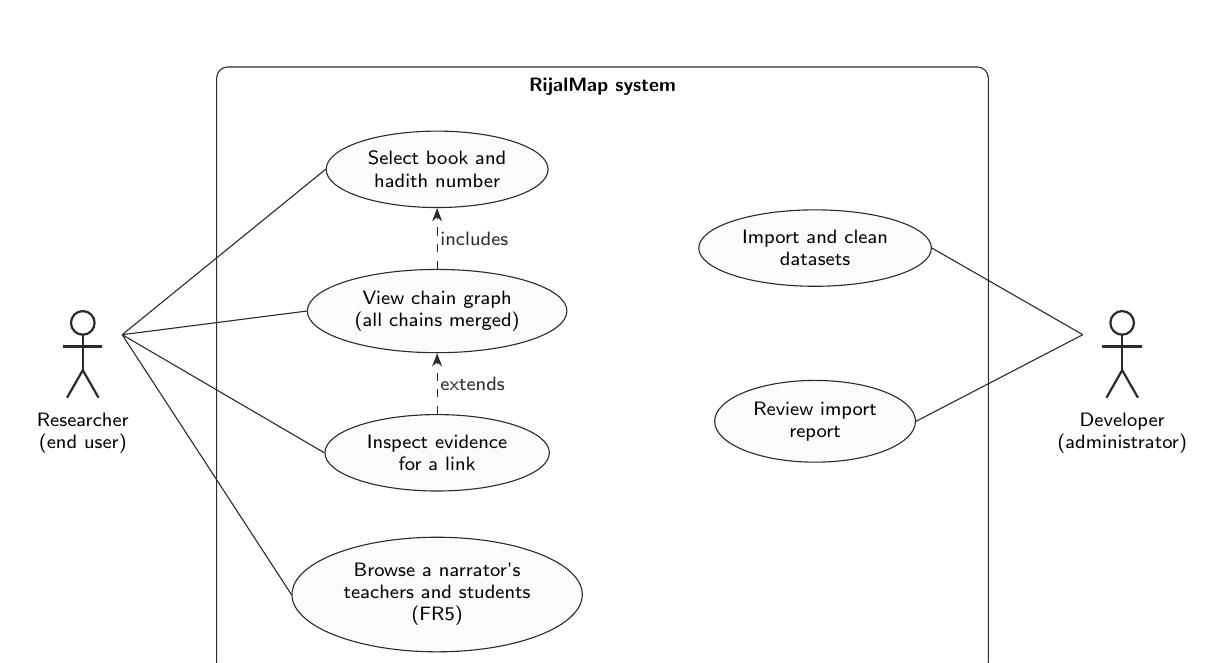
\begin{tikzpicture}
  \draw[ink, rounded corners] (2.6,-1.1) rectangle (12.4,6.6);
  \node[font=\scriptsize\sffamily\bfseries] at (7.5,6.35) {RijalMap system};
  \actor{0.9}{2.4}{Researcher\\ (end user)}
  \actor{14.1}{2.4}{Developer\\ (administrator)}
  \node[draw=ink, ellipse, fill=paper, font=\scriptsize\sffamily, align=center] (u1) at (5.4,5.3) {Select book and\\ hadith number};
  \node[draw=ink, ellipse, fill=paper, font=\scriptsize\sffamily, align=center] (u2) at (5.4,3.5) {View chain graph\\ (all chains merged)};
  \node[draw=ink, ellipse, fill=paper, font=\scriptsize\sffamily, align=center] (u3) at (5.4,1.7) {Inspect evidence\\ for a link};
  \node[draw=ink, ellipse, fill=paper, font=\scriptsize\sffamily, align=center] (u4) at (5.4,-0.1) {Browse a narrator's\\ teachers and students\\ (FR5)};
  \node[draw=ink, ellipse, fill=paper, font=\scriptsize\sffamily, align=center] (u5) at (10.2,4.3) {Import and clean\\ datasets};
  \node[draw=ink, ellipse, fill=paper, font=\scriptsize\sffamily, align=center] (u6) at (10.2,2.1) {Review import\\ report};
  \draw[ink] (1.4,3.2)--(u1.west); \draw[ink] (1.4,3.2)--(u2.west); \draw[ink] (1.4,3.2)--(u3.west); \draw[ink] (1.4,3.2)--(u4.west);
  \draw[ink] (13.6,3.2)--(u5.east); \draw[ink] (13.6,3.2)--(u6.east);
  \draw[dashed, -{Stealth}, ink] (u2.north) -- node[lab, right] {includes} (u1.south);
  \draw[dashed, -{Stealth}, ink] (u3.north) -- node[lab, right] {extends} (u2.south);
\end{tikzpicture}
\caption{Use-case diagram with the two actors.}
\label{fig:usecase}
\end{figure}

\begin{itemize}
  \item \textbf{Researcher (end user):} a student of hadith who wants to see a chain quickly. They choose a collection and number, view the graph, and click links to read the evidence. They only read data and never change it.
  \item \textbf{Developer (administrator):} me. I run the import script that cleans the two CSV files and loads PostgreSQL, and I read the import report (rows loaded, narrator IDs that could not be matched, dates that could not be parsed).
\end{itemize}

\subsection{Database entities and relationships}
Four tables are enough. The chain is stored as an ordered list of narrators, and the links are the consecutive pairs, which the engine computes. This keeps the raw data unchanged and lets one hadith number have several chains, as the dataset does (for example, Jami' al-Tirmidhi no.~1205 appears as three rows with different chains).

\begin{figure}[H]
\centering
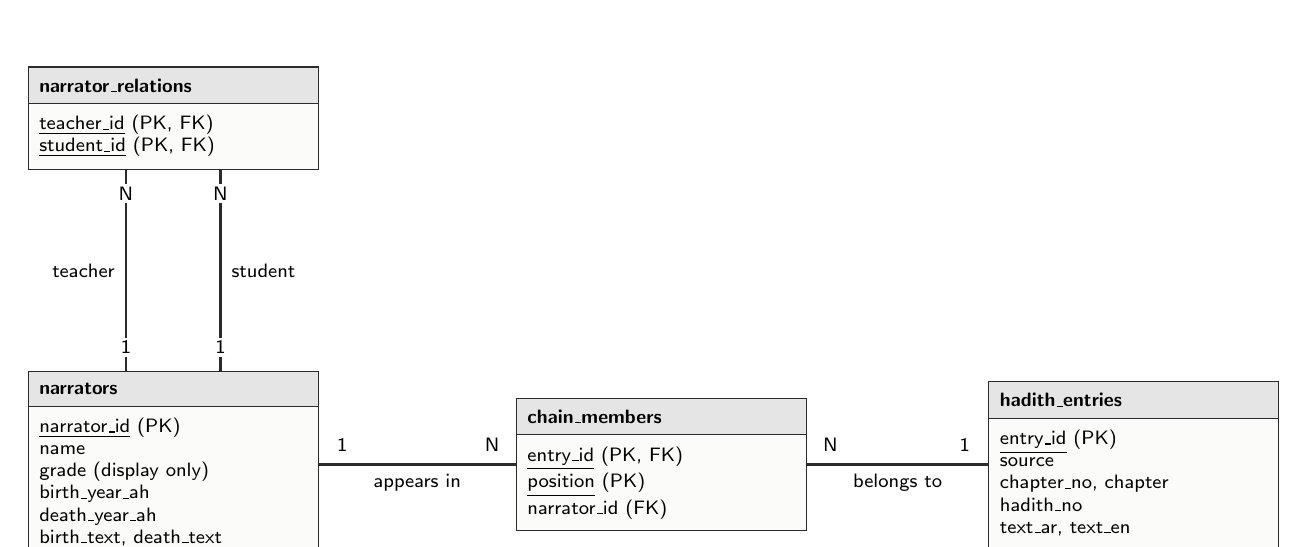
\begin{tikzpicture}
  \node[entity] (rel) at (0,4.4) {\textbf{narrator\_relations}\nodepart{second}\underline{teacher\_id} (PK, FK)\\ \underline{student\_id} (PK, FK)};
  \node[entity] (nar) at (0,0) {\textbf{narrators}\nodepart{second}\underline{narrator\_id} (PK)\\ name\\ grade (display only)\\ birth\_year\_ah\\ death\_year\_ah\\ birth\_text, death\_text};
  \node[entity] (mem) at (6.2,0) {\textbf{chain\_members}\nodepart{second}\underline{entry\_id} (PK, FK)\\ \underline{position} (PK)\\ narrator\_id (FK)};
  \node[entity] (ent) at (12.2,0) {\textbf{hadith\_entries}\nodepart{second}\underline{entry\_id} (PK)\\ source\\ chapter\_no, chapter\\ hadith\_no\\ text\_ar, text\_en};
  % narrator_relations -> narrators (two references)
  \draw[ink, thick] ([xshift=-0.6cm]rel.south) -- ([xshift=-0.6cm]nar.north);
  \draw[ink, thick] ([xshift=0.6cm]rel.south) -- ([xshift=0.6cm]nar.north);
  \node[lab, anchor=east] at ([xshift=-0.7cm]$(rel.south)!0.5!(nar.north)$) {teacher};
  \node[lab, anchor=west] at ([xshift=0.7cm]$(rel.south)!0.5!(nar.north)$) {student};
  \node[lab] at ([xshift=-0.6cm,yshift=-0.3cm]rel.south) {N};
  \node[lab] at ([xshift=0.6cm,yshift=-0.3cm]rel.south) {N};
  \node[lab] at ([xshift=-0.6cm,yshift=0.3cm]nar.north) {1};
  \node[lab] at ([xshift=0.6cm,yshift=0.3cm]nar.north) {1};
  % narrators - chain_members
  \draw[ink, thick] (nar.east) -- (mem.west);
  \node[lab] at ([xshift=0.3cm,yshift=0.25cm]nar.east) {1};
  \node[lab] at ([xshift=-0.3cm,yshift=0.25cm]mem.west) {N};
  \node[font=\scriptsize\sffamily, below] at ($(nar.east)!0.5!(mem.west)$) {appears in};
  % hadith_entries - chain_members
  \draw[ink, thick] (mem.east) -- (ent.west);
  \node[lab] at ([xshift=0.3cm,yshift=0.25cm]mem.east) {N};
  \node[lab] at ([xshift=-0.3cm,yshift=0.25cm]ent.west) {1};
  \node[font=\scriptsize\sffamily, below] at ($(mem.east)!0.5!(ent.west)$) {belongs to};
\end{tikzpicture}
\caption{Entity--relationship diagram (1 = one, N = many). \texttt{narrator\_relations} holds every teacher--student pair listed in either narrator's entry in the dictionary.}
\label{fig:er}
\end{figure}

\begin{itemize}
  \item \textbf{narrators:} one row per dictionary entry; the primary key is the dataset's \texttt{scholar\_indx}. Years are stored in the hijri calendar as signed integers (BH negative), parsed from the text columns.
  \item \textbf{hadith\_entries:} one row per dataset row (one chain each). Several entries can share the same \texttt{(source, hadith\_no)}, which is how multiple chains of one hadith are found.
  \item \textbf{chain\_members:} the ordered narrator list of an entry. A link is the pair of positions $i$ and $i{+}1$ (student, then teacher).
  \item \textbf{narrator\_relations:} the recorded teacher--student pairs, used to decide green versus amber. A composite index on \texttt{(teacher\_id, student\_id)} supports the lookup, and an index on \texttt{(source, hadith\_no)} supports FR1.
\end{itemize}

\subsection{Class structure}
\begin{figure}[H]
\centering
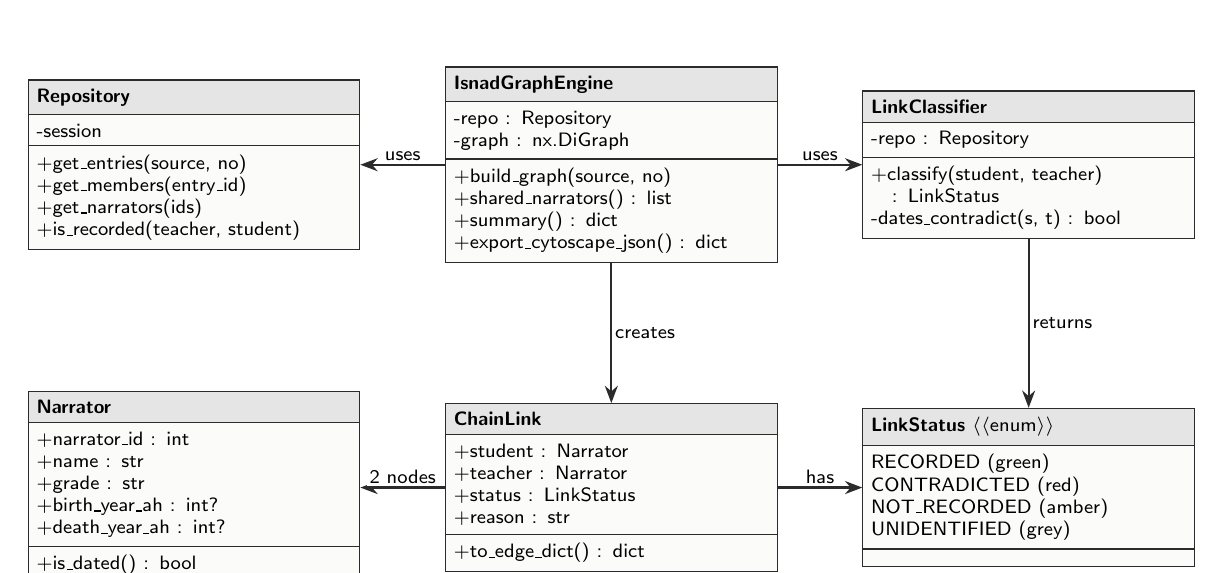
\begin{tikzpicture}
  \node[cls] (repo) at (0,0) {\textbf{Repository}\nodepart{second}-session\nodepart{third}+get\_entries(source, no)\\ +get\_members(entry\_id)\\ +get\_narrators(ids)\\ +is\_recorded(teacher, student)};
  \node[cls] (eng) at (5.3,0) {\textbf{IsnadGraphEngine}\nodepart{second}-repo : Repository\\ -graph : nx.DiGraph\nodepart{third}+build\_graph(source, no)\\ +shared\_narrators() : list\\ +summary() : dict\\ +export\_cytoscape\_json() : dict};
  \node[cls] (clf) at (10.6,0) {\textbf{LinkClassifier}\nodepart{second}-repo : Repository\nodepart{third}+classify(student, teacher)\\ \quad : LinkStatus\\ -dates\_contradict(s, t) : bool};
  \node[cls] (nar) at (0,-4.1) {\textbf{Narrator}\nodepart{second}+narrator\_id : int\\ +name : str\\ +grade : str\\ +birth\_year\_ah : int?\\ +death\_year\_ah : int?\nodepart{third}+is\_dated() : bool};
  \node[cls] (lnk) at (5.3,-4.1) {\textbf{ChainLink}\nodepart{second}+student : Narrator\\ +teacher : Narrator\\ +status : LinkStatus\\ +reason : str\nodepart{third}+to\_edge\_dict() : dict};
  \node[cls] (sta) at (10.6,-4.1) {\textbf{LinkStatus} $\langle\langle$enum$\rangle\rangle$\nodepart{second}RECORDED (green)\\ CONTRADICTED (red)\\ NOT\_RECORDED (amber)\\ UNIDENTIFIED (grey)\nodepart{third}};
  \draw[arr] (eng) -- node[lab, above] {uses} (repo);
  \draw[arr] (eng) -- node[lab, above] {uses} (clf);
  \draw[arr] (clf.south) -- node[lab, right] {returns} (sta.north);
  \draw[arr] (eng.south) -- node[lab, right] {creates} (lnk.north);
  \draw[arr] (lnk.west) -- node[lab, above] {2 nodes} (nar.east);
  \draw[arr] (lnk.east) -- node[lab, above] {has} (sta.west);
\end{tikzpicture}
\caption{Class diagram. The classes follow the tables: \texttt{Narrator} maps to \texttt{narrators}; the engine builds \texttt{ChainLink} objects from \texttt{chain\_members}.}
\label{fig:class}
\end{figure}

This design differs from my proposal's diagram in three ways, which came out of prototyping: the grading attributes are gone, the transmission-edge table is replaced by \texttt{chain\_members} (links are computed, not stored), and classification moved into its own class so it can be tested alone.

\subsection{Link classification logic}
Each consecutive pair (student $S$, teacher $T$) goes through the same four checks in the same order (Figure~\ref{fig:flow}). The order matters: a contradiction by dates beats a dictionary record, and the tooltip will say so when both are present.

\begin{figure}[H]
\centering
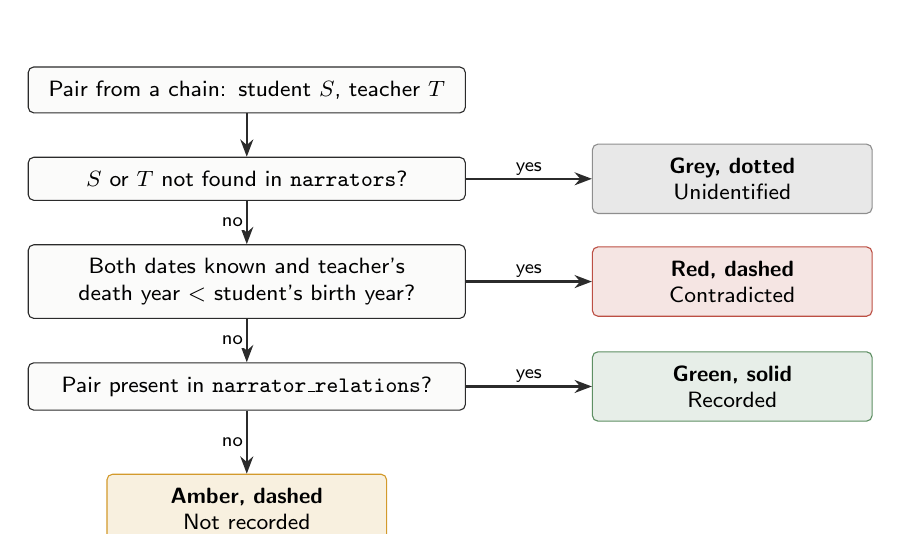
\begin{tikzpicture}[node distance=0.55cm]
  \node[box, text width=5.2cm] (s) {Pair from a chain: student $S$, teacher $T$};
  \node[box, text width=5.2cm, below=of s] (d1) {$S$ or $T$ not found in \texttt{narrators}?};
  \node[box, text width=5.2cm, below=of d1] (d2) {Both dates known and teacher's death year $<$ student's birth year?};
  \node[box, text width=5.2cm, below=of d2] (d3) {Pair present in \texttt{narrator\_relations}?};
  \node[box, text width=3.2cm, right=1.6cm of d1, draw=greyc, fill=greyc!20] (o1) {\textbf{Grey, dotted}\\ Unidentified};
  \node[box, text width=3.2cm, right=1.6cm of d2, draw=terra, fill=terra!15] (o2) {\textbf{Red, dashed}\\ Contradicted};
  \node[box, text width=3.2cm, right=1.6cm of d3, draw=sage, fill=sage!15] (o3) {\textbf{Green, solid}\\ Recorded};
  \node[box, text width=3.2cm, below=0.8cm of d3, draw=amberc, fill=amberc!15] (o4) {\textbf{Amber, dashed}\\ Not recorded};
  \draw[arr] (s)--(d1); \draw[arr] (d1)--node[lab, left] {no}(d2); \draw[arr] (d2)--node[lab, left] {no}(d3);
  \draw[arr] (d3)--node[lab, left] {no}(o4);
  \draw[arr] (d1)--node[lab, above] {yes}(o1); \draw[arr] (d2)--node[lab, above] {yes}(o2); \draw[arr] (d3)--node[lab, above] {yes}(o3);
\end{tikzpicture}
\caption{Decision flow used by \texttt{LinkClassifier.classify()}.}
\label{fig:flow}
\end{figure}

\subsection{Initial wireframes}
Both screens use a light, quiet look: an off-white background, thin borders, and the four muted link colours. The narrator names and statuses in the mock-ups are placeholders to show the layout; they are not output of the system.

\begin{figure}[H]
\centering
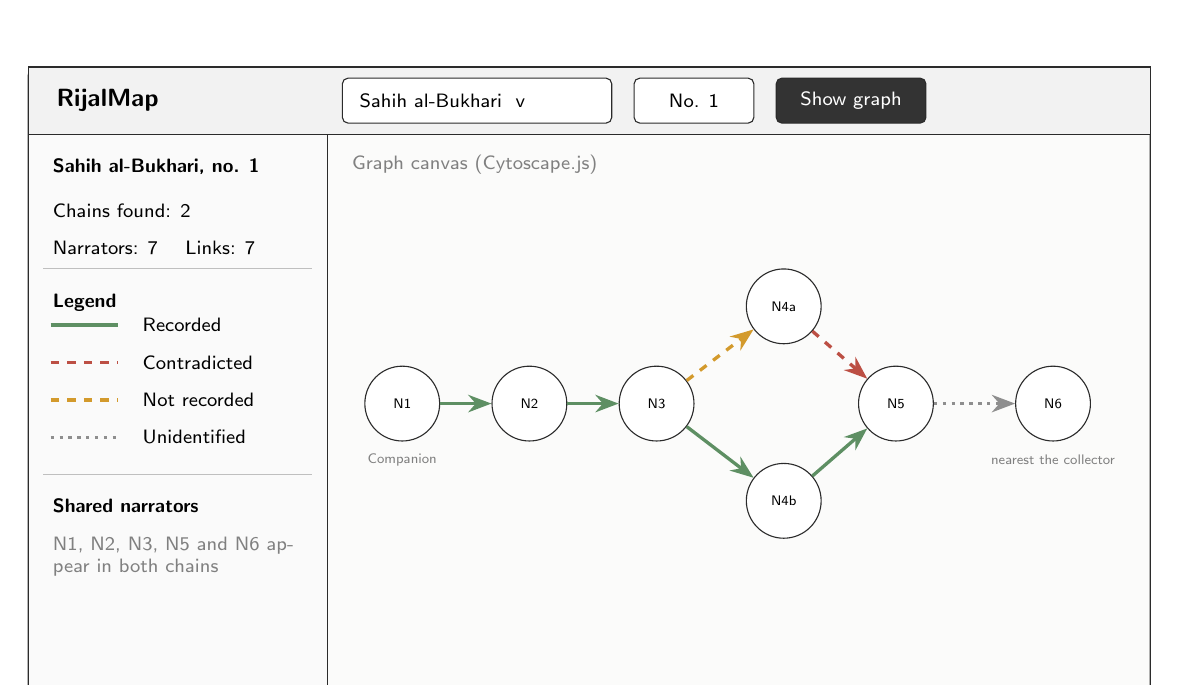
\begin{tikzpicture}[x=0.95cm, y=0.95cm]
  \draw[ink, rounded corners=3pt, fill=paper] (0,0) rectangle (15,8.4);
  \draw[ink, fill=black!5] (0,7.5) rectangle (15,8.4);
  \node[anchor=west, font=\sffamily\bfseries\small] at (0.25,7.95) {RijalMap};
  \draw[ink, rounded corners=2pt, fill=white] (4.2,7.65) rectangle (7.8,8.25);
  \node[anchor=west, font=\sffamily\scriptsize] at (4.3,7.95) {Sahih al-Bukhari \ v};
  \draw[ink, rounded corners=2pt, fill=white] (8.1,7.65) rectangle (9.7,8.25);
  \node[font=\sffamily\scriptsize] at (8.9,7.95) {No. 1};
  \draw[ink, rounded corners=2pt, fill=black!80] (10.0,7.65) rectangle (12.0,8.25);
  \node[font=\sffamily\scriptsize, text=white] at (11.0,7.95) {Show graph};
  % sidebar
  \draw[ink, fill=black!2] (0,0) rectangle (4.0,7.5);
  \node[anchor=north west, font=\sffamily\bfseries\scriptsize] at (0.2,7.3) {Sahih al-Bukhari, no. 1};
  \node[anchor=north west, font=\sffamily\scriptsize] at (0.2,6.7) {Chains found: 2};
  \node[anchor=north west, font=\sffamily\scriptsize] at (0.2,6.2) {Narrators: 7 \quad Links: 7};
  \draw[gray!50] (0.2,5.7)--(3.8,5.7);
  \node[anchor=north west, font=\sffamily\bfseries\scriptsize] at (0.2,5.5) {Legend};
  \draw[sage, very thick] (0.3,4.95)--(1.2,4.95); \node[anchor=west, font=\sffamily\scriptsize] at (1.4,4.95) {Recorded};
  \draw[terra, very thick, dashed] (0.3,4.45)--(1.2,4.45); \node[anchor=west, font=\sffamily\scriptsize] at (1.4,4.45) {Contradicted};
  \draw[amberc, very thick, dashed] (0.3,3.95)--(1.2,3.95); \node[anchor=west, font=\sffamily\scriptsize] at (1.4,3.95) {Not recorded};
  \draw[greyc, very thick, dotted] (0.3,3.45)--(1.2,3.45); \node[anchor=west, font=\sffamily\scriptsize] at (1.4,3.45) {Unidentified};
  \draw[gray!50] (0.2,2.95)--(3.8,2.95);
  \node[anchor=north west, font=\sffamily\bfseries\scriptsize] at (0.2,2.75) {Shared narrators};
  \node[anchor=north west, font=\sffamily\scriptsize, text=gray, text width=3.4cm] at (0.2,2.25) {N1, N2, N3, N5 and N6 appear in both chains};
  % canvas
  \node[anchor=north west, font=\sffamily\scriptsize, text=gray] at (4.2,7.35) {Graph canvas (Cytoscape.js)};
  \node[circle, draw=ink, fill=white, font=\sffamily\tiny, minimum size=0.95cm] (n1) at (5.0,3.9) {N1};
  \node[circle, draw=ink, fill=white, font=\sffamily\tiny, minimum size=0.95cm] (n2) at (6.7,3.9) {N2};
  \node[circle, draw=ink, fill=white, font=\sffamily\tiny, minimum size=0.95cm] (n3) at (8.4,3.9) {N3};
  \node[circle, draw=ink, fill=white, font=\sffamily\tiny, minimum size=0.95cm] (n4) at (10.1,5.2) {N4a};
  \node[circle, draw=ink, fill=white, font=\sffamily\tiny, minimum size=0.95cm] (n4b) at (10.1,2.6) {N4b};
  \node[circle, draw=ink, fill=white, font=\sffamily\tiny, minimum size=0.95cm] (n5) at (11.6,3.9) {N5};
  \node[circle, draw=ink, fill=white, font=\sffamily\tiny, minimum size=0.95cm] (n6) at (13.7,3.9) {N6};
  \draw[-{Stealth}, sage, very thick] (n1)--(n2);
  \draw[-{Stealth}, sage, very thick] (n2)--(n3);
  \draw[-{Stealth}, amberc, very thick, dashed] (n3)--(n4);
  \draw[-{Stealth}, sage, very thick] (n3)--(n4b);
  \draw[-{Stealth}, terra, very thick, dashed] (n4)--(n5);
  \draw[-{Stealth}, sage, very thick] (n4b)--(n5);
  \draw[-{Stealth}, greyc, very thick, dotted] (n5)--(n6);
  \node[font=\sffamily\tiny, text=gray] at (5.0,3.15) {Companion};
  \node[font=\sffamily\tiny, text=gray] at (13.7,3.15) {nearest the collector};
\end{tikzpicture}
\caption{Wireframe 1: main screen. The top bar selects the collection and hadith number; the sidebar summarises the result and shows the legend and narrators shared by several chains; the canvas draws the merged graph, with arrows pointing from teacher to student.}
\label{fig:wire1}
\end{figure}

\begin{figure}[H]
\centering
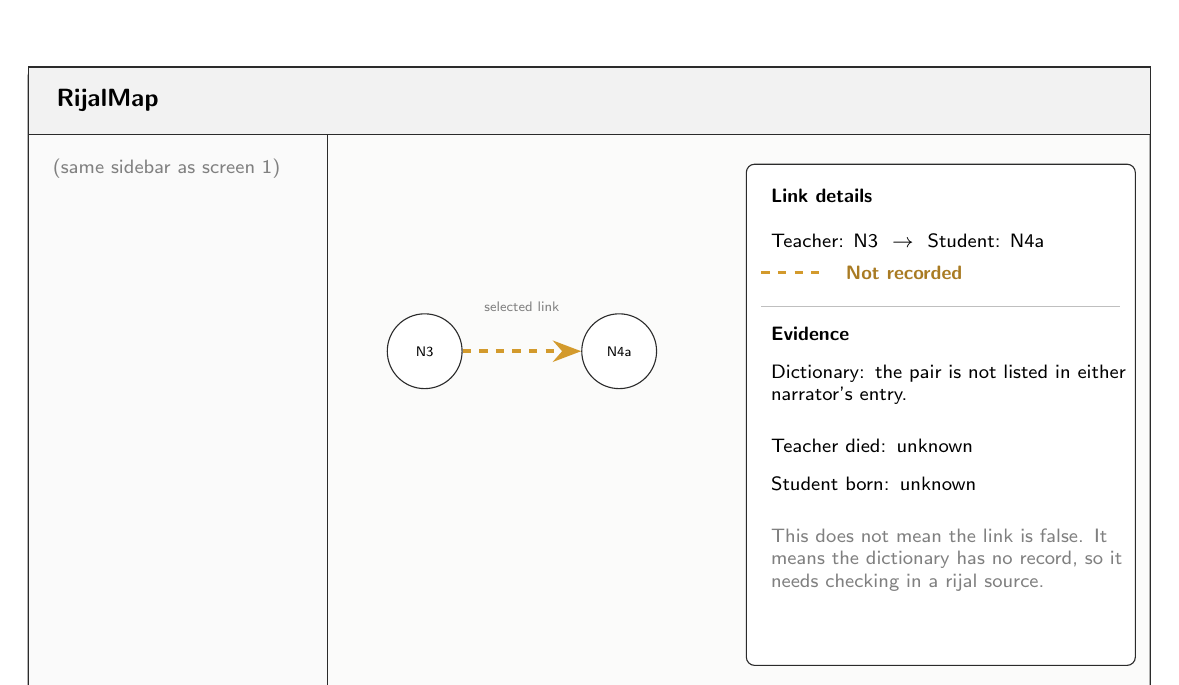
\begin{tikzpicture}[x=0.95cm, y=0.95cm]
  \draw[ink, rounded corners=3pt, fill=paper] (0,0) rectangle (15,8.4);
  \draw[ink, fill=black!5] (0,7.5) rectangle (15,8.4);
  \node[anchor=west, font=\sffamily\bfseries\small] at (0.25,7.95) {RijalMap};
  \draw[ink, fill=black!2] (0,0) rectangle (4.0,7.5);
  \node[anchor=north west, font=\sffamily\scriptsize, text=gray] at (0.2,7.3) {(same sidebar as screen 1)};
  \node[circle, draw=ink, fill=white, font=\sffamily\tiny, minimum size=0.95cm] (n3) at (5.3,4.6) {N3};
  \node[circle, draw=ink, fill=white, font=\sffamily\tiny, minimum size=0.95cm] (n4) at (7.9,4.6) {N4a};
  \draw[-{Stealth}, amberc, ultra thick, dashed] (n3)--(n4);
  \node[font=\sffamily\tiny, text=gray] at (6.6,5.2) {selected link};
  % panel
  \draw[ink, rounded corners=3pt, fill=white] (9.6,0.4) rectangle (14.8,7.1);
  \node[anchor=north west, font=\sffamily\bfseries\scriptsize] at (9.8,6.9) {Link details};
  \node[anchor=north west, font=\sffamily\scriptsize] at (9.8,6.3) {Teacher: N3 \ $\rightarrow$ \ Student: N4a};
  \draw[amberc, very thick, dashed] (9.8,5.65)--(10.6,5.65);
  \node[anchor=west, font=\sffamily\scriptsize\bfseries, text=amberc!80!black] at (10.8,5.65) {Not recorded};
  \draw[gray!50] (9.8,5.2)--(14.6,5.2);
  \node[anchor=north west, font=\sffamily\bfseries\scriptsize] at (9.8,5.05) {Evidence};
  \node[anchor=north west, font=\sffamily\scriptsize, text width=4.6cm] at (9.8,4.55) {Dictionary: the pair is not listed in either narrator's entry.};
  \node[anchor=north west, font=\sffamily\scriptsize, text width=4.6cm] at (9.8,3.55) {Teacher died: unknown};
  \node[anchor=north west, font=\sffamily\scriptsize, text width=4.6cm] at (9.8,3.05) {Student born: unknown};
  \node[anchor=north west, font=\sffamily\scriptsize, text width=4.6cm, text=gray] at (9.8,2.35) {This does not mean the link is false. It means the dictionary has no record, so it needs checking in a rijal source.};
\end{tikzpicture}
\caption{Wireframe 2: after clicking a link, a details panel states the colour, the evidence behind it, and a plain reminder of what the colour does and does not mean.}
\label{fig:wire2}
\end{figure}

\subsection{Major modules and their responsibilities}
\begin{table}[H]
\centering
\small
\begin{tabularx}{\textwidth}{@{}p{2.9cm}Xp{3.0cm}@{}}
\toprule
\textbf{Module} & \textbf{Responsibility} & \textbf{Technology}\\
\midrule
Import & Reads both CSV files, parses narrator IDs and years (BH as negative), builds the four tables, and writes an import report of anything it could not match or parse. Run once by the developer. & Python, pandas, SQLAlchemy\\
Database (Repository) & The only code that talks to PostgreSQL: fetch entries by book and number, fetch narrators, check whether a pair is recorded. & PostgreSQL, SQLAlchemy\\
Graph engine & Builds one directed graph from all chains of the requested hadith, finds narrators shared by several chains, and exports Cytoscape JSON. & Python, NetworkX\\
Link classifier & Applies the decision flow to each pair and returns a status and a reason sentence. & Python\\
API & Exposes the graph and narrator details over HTTP, checks input, and returns clear errors for an unknown book or number. Planned endpoints: list of collections, graph for a hadith, narrator details. & FastAPI\\
Presentation & Collection and number selector, graph canvas, legend, link and narrator details panel. & HTML, JavaScript, Cytoscape.js\\
\bottomrule
\end{tabularx}
\caption{Modules and responsibilities.}
\end{table}

%--------------------------------------------------------------
\section{Known Risks and Limits}
%--------------------------------------------------------------
\begin{itemize}
  \item \textbf{Sparse dates.} Dates are missing for most narrators, so red links will be rare. Most of the colouring will come from the dictionary, which is why the amber state exists.
  \item \textbf{Incomplete or wrong chains.} The hadith dataset's author describes it as an unvalidated draft. A chain in it may omit a narrator, and the tool would then show a break that is really a data error. I will measure this in iteration 5 and tell the user plainly that the colours describe the dataset.
  \item \textbf{Hadith numbering.} The numbers in the dataset may not match the numbering of every printed edition. I will test this on known hadith in iteration 1.
  \item \textbf{What the colours mean.} The tool shows what the data records. It cannot show whether two narrators actually met, and it gives no ruling on a hadith.
\end{itemize}

\begin{thebibliography}{9}
\bibitem{narrators} Fahd (fahd09), \emph{Hadith Narrators Dataset (+24K)}, Kaggle. \url{https://www.kaggle.com/datasets/fahd09/hadith-narrators}
\bibitem{hadiths} Fahd (fahd09), \emph{Hadith Dataset}, Kaggle. \url{https://www.kaggle.com/datasets/fahd09/hadith-dataset}
\end{thebibliography}

\end{document}
